\section{模型的建立与求解}

\subsection{解题思路与流程图}

三个问题共用同一套决策：切图、分核、排序。我们先在问题一上把决策变量、合法性约束和代价结构写成优化模型，问题二、三只修正其中的通信、时间和缓存部分。由于模型中的核内调度、带宽争用和缓存状态都由评估程序模拟，无法直接求出最优解，模型的作用是回答两个问题：代价从哪里来，以及离可达水平还差多少。前者决定构造算法的设计原则，后者用于衡量结果。求解时，对每个（用例，核数）组合由几种构造算法在各自的参数网格上生成候选方案，交给官方评估程序选出最好的一个，再在其上做保持合法性的后处理。整体流程如图~\ref{fig:framework} 所示。

图~\ref{fig:framework} 自上而下分为六层。输入层是计算图、评估程序和单核基准；分析层从测试集结构、性能参照和代价模型三方面给出设计依据，其中代价模型对应问题一、二、三各自的模型建立；构造层是三种构造算法，分别适合多分量、单一巨块和汇聚链三种结构；后处理层包括成组合并、局部搜索、问题二与问题三之间的交叉复评和核数补齐；选优层由官方评估程序在全部候选中取 Makespan 最小者；输出层给出三个问题的方案与指标。三个问题共用构造层和选优层，差别在于代价模型、参数的合适区域和后处理的重点，下文按问题依次展开。

\begin{figure}[H]
  \centering
  % 整体求解流程（正文图 5.1）
\begin{tikzpicture}[x=1mm,y=1mm]
\tikzset{cell/.style={pbox=#1, text width=29mm, minimum height=10mm, font=\footnotesize},
         wide/.style={pbox=#1, minimum height=8mm, font=\footnotesize}}
% 行坐标
\def\yI{0}\def\yA{-15}\def\yC{-31}\def\yP{-48}\def\yS{-62}\def\yO{-76}
% ---- 输入
\node[pio, trapezium stretches body, text width=24mm, minimum width=30mm, minimum height=10mm, font=\footnotesize] (i1) at (17,\yI) {计算图 $G$\\100 个用例};
\node[pio, trapezium stretches body, text width=24mm, minimum width=30mm, minimum height=10mm, font=\footnotesize] (i2) at (53,\yI) {官方评估程序\\$E_p$};
\node[pio, trapezium stretches body, text width=24mm, minimum width=30mm, minimum height=10mm, font=\footnotesize] (i3) at (89,\yI) {单核基准\\$M_1^{\mathrm{sc}}$};
% ---- 分析
\node[cell=cA] (a1) at (17,\yA) {结构刻画\\$\eta$，$\omega$};
\node[cell=cA] (a2) at (53,\yA) {性能参照\\$\underline{M}_k^{\mathrm{an}}$，$M_k^0$，$M_k^\delta$};
\node[cell=cA] (a3) at (89,\yA) {代价模型\\$Q_A,\ Q_B,\ h,\ \theta$};
% ---- 构造
\node[cell=cB] (c1) at (17,\yC) {$\mathrm{LPT}(\alpha)$\\多分量};
\node[cell=cB] (c2) at (53,\yC) {$\mathrm{BAND}(W)$\\单一巨块};
\node[cell=cB] (c3) at (89,\yC) {$\mathrm{PHASE}(\lambda)$\\汇聚链};
% ---- 后处理
\node[pbox=cO, text width=21mm, minimum height=9mm, font=\footnotesize] (p1) at (10,\yP) {成组合并};
\node[pbox=cO, text width=21mm, minimum height=9mm, font=\footnotesize] (p2) at (38,\yP) {局部搜索};
\node[pbox=cO, text width=21mm, minimum height=9mm, font=\footnotesize] (p3) at (66,\yP) {交叉复评\\问题二$\leftrightarrow$三};
\node[pbox=cO, text width=21mm, minimum height=9mm, font=\footnotesize] (p4) at (94,\yP) {核数补齐};
% ---- 选优
\node[wide=cA, text width=100mm] (s) at (53,\yS) {$x^*=\argmin_{x\in\mathcal{C}_{p,k}}E_p(x)$};
% ---- 输出
\node[pio, trapezium stretches body, text width=24mm, minimum width=30mm, minimum height=10mm, font=\footnotesize] (o1) at (17,\yO) {问题一\\场景 A};
\node[pio, trapezium stretches body, text width=24mm, minimum width=30mm, minimum height=10mm, font=\footnotesize] (o2) at (53,\yO) {问题二\\场景 B};
\node[pio, trapezium stretches body, text width=24mm, minimum width=30mm, minimum height=10mm, font=\footnotesize] (o3) at (89,\yO) {问题三\\只读 L2};
% ---- 箭头
\foreach \a/\b in {i1/a1,i2/a2,i3/a3,a1/c1,a2/c2,a3/c3} \draw[parr] (\a) -- (\b);
\coordinate (bus) at (53,\yP+8);
\foreach \c in {c1,c2,c3} \draw[line width=0.7pt, draw=ink2] (\c.south) -- (\c.south |- bus);
\draw[line width=0.7pt, draw=ink2] (10,\yP+8) -- (94,\yP+8);
\foreach \p in {p1,p2,p3,p4} \draw[parr] (\p.north |- bus) -- (\p.north);
\foreach \p in {p1,p2,p3,p4} \draw[parr] (\p.south) -- (\p.south |- s.north);
\foreach \o in {o1,o2,o3} \draw[parr] (s.south -| \o) -- (\o.north);
% ---- 层标签
\foreach \y/\t in {\yI/输入, \yA/分析, \yC/构造, \yP/后处理, \yS/选优, \yO/输出}
  \node[plab, anchor=east, font=\footnotesize\bfseries] at (-3,\y) {\t};
\end{tikzpicture}

  \caption{整体求解流程}
  \label{fig:framework}
\end{figure}

\subsubsection{测试集的结构特征}\label{sec:data-struct}

题目给出 100 张计算图。可分配操作数从 \V{ops_min} 到 \V{ops_max}，中位数 \V{ops_median}；官方单核基准的 Makespan 从 \V{single_min} 到 \V{single_max} 周期，相差三个多数量级。规模差别这么大，同一个参数不可能对所有用例都合适，这是后文逐用例选优的直接原因。为了刻画结构，先构造操作依赖图 $D=(\Oe,A)$：对 $u,v\in\Oe$，若原图中存在从 $u$ 到 $v$ 的有向路径，且中间节点只有张量或 COPY 节点，则 $(u,v)\in A$。$D$ 是可分配操作之间真正的依赖关系，后文的构造算法都在 $D$ 上进行。用两个量描述 $D$ 的形状：
\begin{equation}
  \eta = \frac{\max_{C}\ \sum_{v\in C} c_v}{\sum_{v\in \Oe} c_v},\qquad
  \omega = \frac{W_M+W_V}{L_{\mathrm{cp}}},
  \label{eq:eta-omega}
\end{equation}
其中 $C$ 取遍 $D$ 的弱连通分量。$\eta$ 是最大分量占全部计算量的比例，$\omega$ 是平均每一时刻可以同时推进的计算量，称为宽度比。

按 $\eta$ 把用例分为三类：单一巨块（$\eta>0.8$，记为 I 类）、主块加碎片（$0.3\le\eta\le 0.8$，II 类）和多分量（$\eta<0.3$，III 类），分别有 \V{family_count_I}、\V{family_count_II}、\V{family_count_III} 个用例。分布见图~\ref{fig:dataset}。宽度比的中位数为 \V{width_ratio_median}，即使是 I 类，宽度比中位数也有 \V{famI_width_median}，说明从依赖结构看，绝大多数计算图都可以充分并行；难点在于 I 类图的并行性藏在同一个连通分量内部，不能靠“不同分量放不同核心”获得。

\begin{figure}[H]
  \centering
  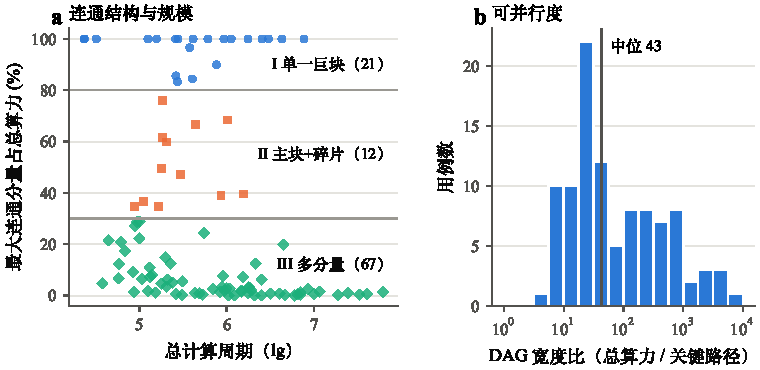
\includegraphics[width=\textwidth]{dataset_profile}
  \caption{测试集结构。(a) 最大弱连通分量的计算量占比 $\eta$ 与类别划分；(b) 宽度比 $\omega$ 的分布}
  \label{fig:dataset}
\end{figure}

\subsubsection{评价口径与性能参照}\label{sec:refs}

按题目定义，$k$ 核加速比为
\begin{equation}
  \rho_k=\frac{M_1^{\mathrm{sc}}}{M_k},\qquad \rho_1\equiv 1,
  \label{eq:speedup}
\end{equation}
其中 $M_1^{\mathrm{sc}}$ 是把整张图作为一个 Task 交给核内调度器得到的 Makespan，平均加速比取 100 个用例的算术平均。这个基准本身包含可以避免的开销：整张大图作为一个 Task 时，L1/UB 放不下全部中间张量，核内调度器会插入大量换入换出，而切成子图后每个子图的工作集变小，换出也随之减少。所以把图切开即使只用一个核也可能更快，$\rho_k>k$ 的超线性情形会出现。另外，题目附带的示例生成器 \texttt{stub\_multicore\_cut\_and\_schedule.py} 只生成格式合法的随机方案，以 case\_010 为例，它的 4 核方案 Makespan 为 88{,}416，比单核基准 86{,}969 还慢。用它作对照会高估算法效果，本文的对照基线一律采用第~\ref{sec:lpt} 节的分量装箱（$\alpha=0.25$），称为朴素基线。

只报告加速比，看不出离可达水平还有多远。我们用三个逐步收紧的参照值来衡量。第一个是解析下界：任何 $k$ 核方案都要完成全部计算、走完关键路径，并至少搬运一遍图的输入与输出，因此
\begin{equation}
  \underline{M}_k^{\mathrm{an}}=\max\left\{L_{\mathrm{cp}},\ \frac{W_M}{k},\ \frac{W_V}{k},\ \frac{Q_{\min}}{B}\right\},
  \label{eq:lb-analytic}
\end{equation}
$Q_{\min}$ 为图输入张量与输出张量的字节数之和。四项分别对应四个必须满足的条件：关键路径上的操作只能依次执行，所以 Makespan 不小于 $L_{\mathrm{cp}}$；全部 Cube 计算要分给 $k$ 个核心的 Cube 单元完成，负载最均衡时每个核心也要承担 $W_M/k$，Vector 同理；图的输入至少读入一次、输出至少写出一次，这些字节共享带宽 $B$，至少需要 $Q_{\min}/B$ 周期。Makespan 不小于其中任何一项，因而不小于它们的最大值。在忽略同步与换出的意义下，它是 Makespan 的下界，1 核时对应的平均加速比已达 \V{lb_k1_speedup_mean}，这也印证了单核基准中换出开销之大。第二个是零通信表调度：在 $D$ 上为每个核心设四条流水线，操作在前驱全部完成且对应流水线空闲时尽早开始，通信代价置零，所得 Makespan 记为 $M_k^0$，理想并行效率为
\begin{equation}
  \varepsilon_k=\frac{M_1^{0}}{k\,M_k^{0}}.
  \label{eq:ideal-eff}
\end{equation}
若依赖不构成任何限制，$k$ 核可以把单核的工作完全平分，$M_k^0=M_1^0/k$，效率为 1；依赖使部分核心在等待前驱时空闲，$M_k^0$ 大于 $M_1^0/k$，效率随之小于 1。所以 $\varepsilon_k$ 衡量的是依赖结构本身造成的并行损失。4 核时 $\varepsilon_4$ 的均值为 \V{ideal_k4_eff_mean}，只有 \V{ideal_k4_eff_lt50} 个用例低于 50\%，说明依赖结构本身几乎不限制并行，限制并行的是通信与同步。

第三个是含同步代价的可达参考。在同一表调度中加入固定的跨核延迟 $\delta$：操作 $v$ 放在核心 $n$ 上的最早开始时刻为
\begin{equation}
  \mathrm{EST}(v,n)=\max\Big\{\,\mathrm{avail}\big(n,\pi(v)\big),\ \max_{(u,v)\in A}\big(f_u+\delta_{un}\big)\Big\},\qquad
  \delta_{un}=\begin{cases}\delta, & \core(u)\ne n,\\ 0, & \core(u)=n,\end{cases}
  \label{eq:est-sync}
\end{equation}
其中 $\mathrm{avail}(n,p)$ 为核心 $n$ 上流水线 $p$ 的空闲时刻。$v$ 能开始，需要它所在的流水线已经空闲，并且所有前驱的结果都已可用：同核前驱完成即可用，跨核前驱还要再等 $\delta$ 周期，两者取最大就是最早开始时刻。就绪操作按自底向上关键路径长度降序处理，每个操作贪心地放到使 $\mathrm{EST}(v,n)+c_v$ 最小的核心；场景 A 取 $\delta=\delta_{\mathrm{cross}}$，场景 B 取 $\delta=\delta_B$。所得 Makespan 记为 $M_k^{\delta}$，本文结果对它的达成率定义为
\begin{equation}
  \mathrm{ach}_k=\frac{M_k^{\delta}}{M_k},
  \label{eq:achieve}
\end{equation}
它等于可达参考加速比 $M_1^{\mathrm{sc}}/M_k^{\delta}$ 与本文加速比 $M_1^{\mathrm{sc}}/M_k$ 之比，分子分母中的 $M_1^{\mathrm{sc}}$ 相互抵消，所以与单核基准无关。这一参照仍然忽略 DDR 争用和缓存换出，但计入了对小图影响最大的固定同步延迟。它是贪心结果，不是严格上界，实测结果可能超过它。三个参照值的平均加速比见表~\ref{tab:refs}，在各核数下依次递减，与逐步加入约束的构造一致。解析下界含搬运项而表调度不含，个别以搬运为主的用例上两者大小可能相反，这里的递减只就均值而言。从零通信到含同步，4 核平均加速比从 \V{p1_k4_ideal0_speedup_mean} 降到 \V{p1_k4_ref_speedup_mean}（场景 A），差的正是固定同步延迟的代价；对理想 Makespan 只有几千周期的小图，十几条跨核依赖链就能吃掉大部分并行收益。

\begin{table}[H]
\centering
\caption{性能参照的平均加速比（100 个用例）}
\label{tab:refs}
\renewcommand\arraystretch{1.15}
\begin{tabular}{lcccc}
\toprule
参照 & 2 核 & 3 核 & 4 核 & 5 核 \\
\midrule
解析下界，式 \eqref{eq:lb-analytic} & \V{lb_k2_speedup_mean} & \V{lb_k3_speedup_mean} & \V{lb_k4_speedup_mean} & \V{lb_k5_speedup_mean} \\
零通信表调度 & \V{p1_k2_ideal0_speedup_mean} & \V{p1_k3_ideal0_speedup_mean} & \V{p1_k4_ideal0_speedup_mean} & \V{p1_k5_ideal0_speedup_mean} \\
含同步可达参考，场景 A（$\delta=1000$） & \V{p1_k2_ref_speedup_mean} & \V{p1_k3_ref_speedup_mean} & \V{p1_k4_ref_speedup_mean} & \V{p1_k5_ref_speedup_mean} \\
含同步可达参考，场景 B（$\delta=500$） & \V{p2_k2_ref_speedup_mean} & \V{p2_k3_ref_speedup_mean} & \V{p2_k4_ref_speedup_mean} & \V{p2_k5_ref_speedup_mean} \\
\bottomrule
\end{tabular}
\end{table}
